\chapter{Theoretical Background}
In this chapter we give a introduction in various topics and areas which are necessary in order to understand the implementation of our pipeline and how its generated results were computed. 

\section{Optical Flow}
\label{sec:optical_flow}
In this section we explain the principles and the idea behind the optical flow. We emphasize this concept by giving an in intuitive definition, followed by a mathematical definition. Next, we discuss how such flow fields can be visualized. Lastly, we summarize and explain the pioneering formulation of HS used to estimate flow fields.

\subsection{Definition}

The optical flow is a visual phenomenon that describes the perception of motion.
By definition, it is the apparent visual motion a moving viewer experiences.

To To give the reader a better, more intuitive understanding of this concept, have a look at figure $\ref{fig:motion_eg}$.
\begin{figure}[H]
\begin{center}
\subfigure[1st Frame]{
   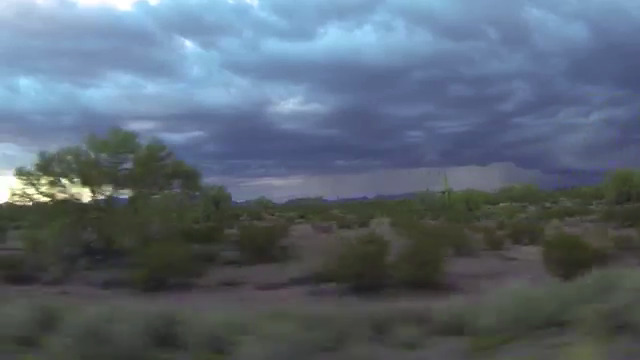
\includegraphics[width=0.47\linewidth] {background/of/ls1}
   \label{fig:motion_eg_f1}
}
\subfigure[2nd Frame]{
   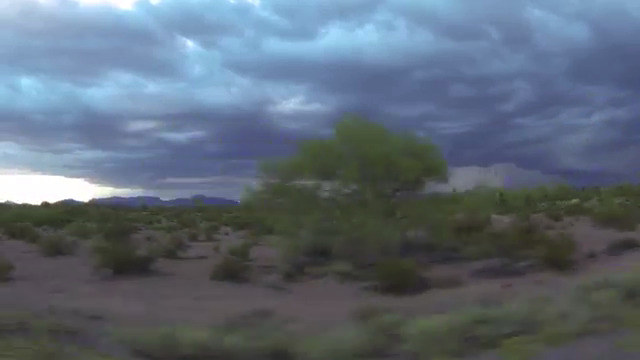
\includegraphics[width=0.47\linewidth] {background/of/ls2}
   \label{fig:motion_eg_f2}
}
~
\subfigure[3rd Frame]{
   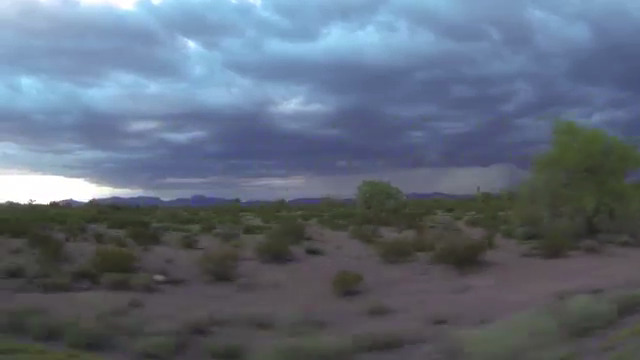
\includegraphics[width=0.47\linewidth] {background/of/ls3}
   \label{fig:motion_eg_f3}
}
\subfigure[4th Frame]{
   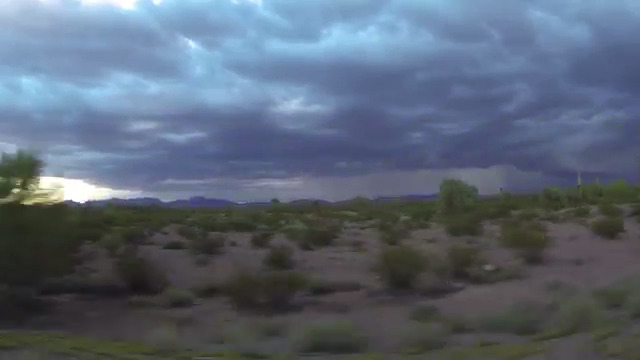
\includegraphics[width=0.47\linewidth] {background/of/ls4}
   \label{fig:motion_eg_f4}
}
\end{center}
\caption[Motion Example]{An example$\footnotemark$ of motion effects illustrated by four frames of a video sequence. Objects far away in the background, such as the mountain or the clouds seems to stand still. Objects being a fair distant apart, but also not too far away can be seen over several frames, such as the tree, that is passed. In addition, we also see observe, that the tree moves along the opposite direction as the driving car. Last, we also see the effect of motion blur for objects that are very close such as the grass.}
\label{fig:motion_eg}
\end{figure}
\footnotetext{The shown frames have been extracted from the following youtube video: \\ \url{https://www.youtube.com/watch?v=lo-pWLmMagc}}
Imagine you sit in a moving car and you are looking out of its windows. While doing so, you will observe that every overtaken object appear to move backwards. Furthermore, objects far in the background seem to stand still, whereas object close to the train seem to move very fast and thus have a blurry look. Therefore, the optical flow is an indicator for distance and size of an object. Moreover, the angle between the observer's viewing direction and the direction of the moving influences the optical flow. if an object travels perpendicular to the train or is directly above or below the it, then the optical flow is maximal. Lastly, an objects directly in front of a viewer will not exhibit any optical flow and thus appear to stand still. However, since not the whole object silhouette is directly in front of the viewer, its edges appear to move and therefore, the such an object appears to get either get larger or smaller, depending on its moving direction.

In summary, the optical flow has the following key properties:
\begin{itemize}
  \item Overtaken objects appear to move backwards.
  \item Distant objects seem to move very slowly and close objects appear to move fast.
  \item The magnitude of the optical flow is doubles if either the speed of the traveling viewer is doubled or the distance to the observed object is halved.
  \item The optical flow varies depending on the angle between the viewing direction and and the direction of movement of the observed object.
  \item The optical flow is maximal if either the object is moving orthogonally towards the viewer's direction or it is moving directly above or below it.
  \item Objects directly in front of a viewer exhibit no optical flow.
\end{itemize}

The underlying basis input of our whole approach depicts the optical flow, computed from a given inputs sequence.

%TODO: Write mathematical definition of the optical flow
\subsection{Mathematical Formulation}


The optical flow is a vector field that defines a point-to-point correspondence between two successive frames. Each vector acts as the displacement of a point in the first frame to match its corresponding point in the second frame.
\subsection{Visualization of Flowfields}

For visualizing flow fields we use the color encoding shown in subfigure $\ref{fig:color_encoding_flows_a}$. The shown color plate provides color values for the normalized flow vectors. The angle in the circle corresponds to the direction and the distance to the center to the velocity. \\ \\
Figure $\ref{fig:color_encoding_flows}$ also contains an example of a flow visualization using these color codes.
\begin{figure}[H]
\begin{center}
\subfigure[Flow Color Codes]{
   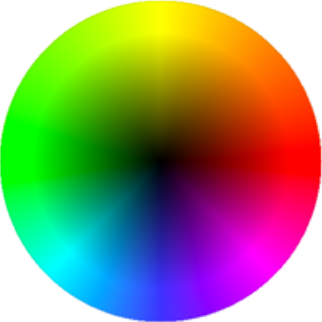
\includegraphics[width=0.35\linewidth] {background/of/flowfield_color_encoding}
   \label{fig:color_encoding_flows_a}
}
~
\subfigure[Example flow visualization]{
   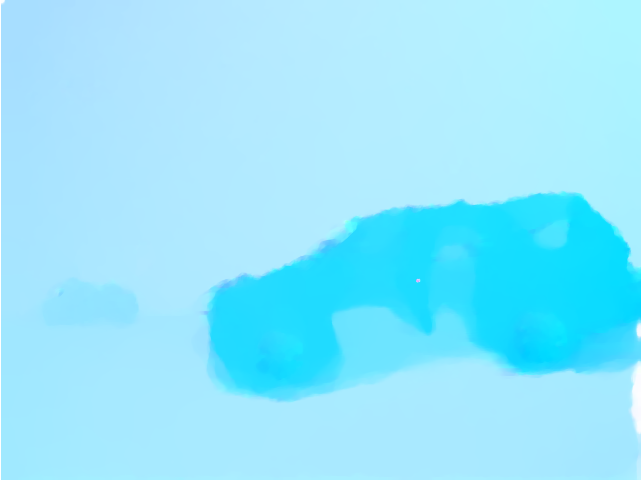
\includegraphics[width=0.5\linewidth] {background/of/cars_fwf_1}
   \label{fig:color_encoding_flows_b}
}
\end{center}
\caption[Visual Color Encoding of Flow Fields]{On the left a visualization of the color plate used to draw flow fields and on the right flow field visualized by this color scheme.}
\label{fig:color_encoding_flows}
\end{figure}

\subsection{Original Flow Estimation Method of H.S.}
\label{sec:hs_formulation}
In the pioneering work of $\cite{Hs81}$ B. Horn and B. Schnunck describe a technique to estimate the optical flow. Back then they defined the optical flow as the distribution of apparent velocities of movement of brightness patterns in an image. \\ \\
Moreover, they already understood the potential of the optical flow and stated the following properties: Can arise from relative motion of objects and the viewer and provide information about the spatial arrangement of the viewed objects and the rate of change in that arrangement. Discontinuities in the optical flow can help to perform segmentation tasks. \\ \\
Sticking to their flow definition they derived an equation that relates the change in the image brightness at a point to the motion of the brightness. \\ \\
Their formulation is based on the following assumptions:
\begin{itemize}
  \item The surface is assumed to be flat. This avoids brightness variations due to shading effects.
  \item The incident illumination is uniform across the surface. Then, the brightness at a point in the image is proportional to the reflectance of the surface at the corresponding point on the object.
  \item The Reflectance varies smoothly and has no spatial discontinuities. Having no discontinuities assures that the image brightness is differentiable.
  \item Situations where objects occlude one another are excluded.
\end{itemize}
These assumptions allow to conclude, that in their model the brightness of a particular point in the pattern is constant. \\ \\
Let the image brightness at a point $(x,y)$ in the image plane at time $t$ be denoted by $E(x,y,t)$. Since the brightness of any point is constant, $\frac{d E}{dt} = 0$ hold true. Using the chain rule for differentiation, they derived the expression in equation $\ref{eq:flow_eq}$.  
\begin{equation}
\begin{aligned}
0 &= \frac{d E}{dt} \\
&= \frac{\partial E}{\partial x} \frac{x}{dt} + \frac{\partial E}{\partial y} \frac{y}{dt} + \frac{\partial E}{\partial t} \\
&= E_{x} u + E_{y} v + E_{t}
\end{aligned}
\label{eq:flow_eq}	
\end{equation}
where we the following substitutions were used to derive the last identity of equation $\ref{eq:flow_eq}$:
\begin{equation}
\begin{aligned}
	u = \frac{dx}{dt} \text{ and } v = \frac{dy}{dt}
\end{aligned}
\end{equation}
By re-ordering the terms of equation $\ref{eq:flow_eq}$ the same way like it has been done in equation $\ref{eq:reordered_flow_eq}$:
\begin{equation}
\begin{aligned}
	(E_x, E_y) \cdot (u, v) &= -E_t \\
	\underbrace{-\frac{1}{E_t}\left( E_x, E_y \right)}_\text{known} \cdot \underbrace{(u, v)}_\text{unknown} &= 1
\end{aligned}
\label{eq:reordered_flow_eq}
\end{equation}
Hence, they could show that the change in image brightness can be formulated by a single linear equations with two unknowns $u$ and $v$, the so called $\textit{flow velocity}$. As a consequence, such a flow velocity cannot be computed locally without introducing additional constraints.



\section{General Motion Segmentation Pipeline}
motion segmentation aims at decomposing a video in moving objects and background by segmenting the objects that undergo different motion patterns.

In this section we describe a conceptual approach how the motion segmentation task using optical flows is commonly approached in literature. 

\section{Spectral Clustering}
Kernighan-Lin Heuristic, Graph Cut
multi-label CRF on superpixels for class segmentation $\cite{Fulkerson2009}$

$\cite{Ker70}$

%TODO: maybe we should introduce a section called filtering, containing bilateral filtering, harris corner detector and so forth..
\section{Harris Corner Detector}
\label{sec:harris_corner_detector}

% TODO state idea of an edge

Let us consider a grayscale image $I$. We are going to sweep a window $w(x,y)$ (with displacements u in the x direction and v in the right direction) I and will calculate the variation of intensity. Since we are looking for windows with corners, we are looking for windows with a large variation in intensity. Hence, we have to maximize the equation above, specifically the term:
\begin{equation}
	E \left( u, v \right) = \sum_{x,y} w \left( x,y \right) \left[ I(x + u, y + v) - I(x, y) \right]^2
\label{eq:var_intensitiy_def}
\end{equation}
Next, the term $I(x + u, y + v)$ is expressed by the first order taylor series expansion as the follows:
\begin{equation}
	I(x + u, y + v) = I(x,y) + u I_x (x, y) + v I_y (x,y) + \text{h.o.t}
\label{eq:taylor_exp_intensity}
\end{equation}
Next, we put the first order approximation of equation $\ref{eq:taylor_exp_intensity}$ into equation $\ref{eq:var_intensitiy_def}$ to simplify the definition of $E$.
\begin{equation}
\begin{aligned}
E \left( u, v \right) 
&= \sum_{x,y} w \left( x,y \right) \left[ I(x + u, y + v) - I(x, y) \right]^2 \\
&\approx \sum_{x,y} w \left( x,y \right) \left[ I(x,y) + u I_x (x, y) + v I_y (x,y) - I(x, y) \right]^2 \\
&= \sum_{x,y} w \left( x,y \right) \left[ u I_x (x, y) + v I_y (x,y) \right]^2 \\
&= \sum_{x,y} w \left( x,y \right) u^2 I_x^2 + 2 u v I_x I_y v^2 I_y^2 \\
&= \left( u,v \right) \left( \sum_{x,y} w (x,y)
\begin{pmatrix}
I_x^2 & I_x I_y \\
I_x I_y & I_y^2 \\
\end{pmatrix}
\right) \colvec{u}{v}
\end{aligned}
\label{eq:var_intensitiy_developed}
\end{equation}
Let us define the following substitution
\begin{equation}
M = \sum_{x,y} w  (x,y)
\begin{pmatrix}
I_x^2 & I_x I_y \\
I_y^2 & I_x I_y \\
\end{pmatrix}
\label{eq:var_intensity_sub}
\end{equation}
Putting the substitution from equation $\ref{eq:var_intensity_sub}$ into the final form of equation $\ref{eq:var_intensitiy_developed}$ we obtain the final form
\begin{equation}
	E \left( u, v \right) \approx \left( u,v \right) M \colvec{u}{v}
\end{equation}.
A score is calculated for each window, to determine if it can possibly contain a corner:
\begin{equation}
\begin{aligned}
& R = \det(M) - \kappa \left(\text{trace}(M)\right)^2 \\
&\text{where } \det(M) = \lambda_1 \lambda_2 \text{ and } \text{trace}(M) = \lambda_1 + \lambda_2
\end{aligned}
\label{eq:harris_response}
\end{equation}

\section{Camera Calibrations}
explain pinhole model
explain from scene to camera-space to image-space
mention focal length, principal point
mention how depth could be incooperated
explain intrinsic,extrinsic calibrations

\section{Bilateral Filter}

\section{K-Means}





